%%%%%%%%%%%%%%%%%%%%%%%%%%%%%%%%%%%%%%%%%%%%%%%%%%%%%%%%%%%%%%%%%%%%%%%%%%
 %																		%
 %	Plantilla Latex para presentación del proyecto de curso				%
 %	Programación de Aplicaciones para Internet y la Nube					%
 %																		%
 %	Creada por: Duván Pardo, Wilson López								%
 %																		%
 %	Versión: 0.1															%
 %	Dapardoc@gmail.com ; Wilrilo@gmail.com								%
 %																		% 
 %	Se requieren los archivos plantilla.bbl y							% 
 %	El directorio Imagenes que contiene: CECAD,DC, Elementos y RITA		%  
 %																		%
%%%%%%%%%%%%%%%%%%%%%%%%%%%%%%%%%%%%%%%%%%%%%%%%%%%%%%%%%%%%%%%%%%%%%%%%%%

\documentclass[10pt]{article}   			% Describe el tipo de documento, y el tamaño de la letra del texto

\usepackage[utf8]{inputenc}				% Define codificación para que permita caracteres latinos (acentos)
\usepackage[spanish,activeacute]{babel} 	% Paquete para poder escribir con tildes y otros caracteres especiales

\usepackage{vmargin}						% Código para margenes y formato de página
\setpapersize{A4}
\setmargins	{2.2cm}     					% margen izquierdo
			{1 cm}                 		% margen superior
			{16.5cm}               		% anchura del texto
			{23.42cm}             		% altura del texto
			{20pt}                		% altura de los encabezados
			{1.2cm}               		% espacio entre el texto y los encabezados
			{0pt}                		% altura del pie de página
			{2cm}                 		% espacio entre el texto y el pie de página

\usepackage{amsmath}						% paquete para expresiones matemáticas
\usepackage{amsfonts}					% paquete para escritura de ecuaciones 
\usepackage{amssymb}						% paquete para caracteres especiales para ecuaciones 

\usepackage{fancyhdr}					% Temas para encabezado y pie de pagina
\usepackage{fancyvrb}
\pagestyle{fancy} 

\pagenumbering{arabic} 					% Numeración de paginas {arabic roman}
\usepackage{hyperref}					% Para hipervinculos
\usepackage{graphicx}					% Para incluir imágenes
\usepackage{float}	
\usepackage{caption}						% Descripciones de las figuras

\usepackage{subcaption}					% Descripción varias imagenes en usa sola figura
\graphicspath{ {Imagenes/} }				% Directorio de imágenes esta capeta va donde esta el archivo tex


\usepackage{color, colortbl}				% Colores para tablas
\usepackage{listings}					% Para el código Fuente
\usepackage{xcolor}						% para color en codigos o listrings
\definecolor{limegreen}{RGB}{50,100,50}	% Definición de colores ejemplo verde en RGB
\definecolor{Red}{RGB}{220,120,120}		% se definen colores para la tabla en el cronograma pueden ser RGB 0-255 o rgb 0-1 cada componente
\definecolor{LightCyan}{rgb}{0.88,1,1}
\definecolor{azul}{RGB}{120,120,210}
\lstdefinestyle{base}{
	language=C,
	emptylines=1,
	breaklines=true,
	showspaces=fasle,
	showstringspaces=false,
	extendedchars=true,
	basicstyle=\ttfamily\color{black},
	moredelim=**[is][\color{limegreen}]{'}{'}, 	% Para este caso especial el caracter ' y & encierran
	moredelim=**[is][\color{blue}]{&}{&},		% un fragmento de código que quiere ser coloreado
}

\lstset{numbers=left, numberstyle=\tiny, stepnumber=2, numbersep=5pt}

%Aquí inicia el documento.
\begin{document}
	% Se define el Encabezado
	%clhead[]{Proyecto}
	\lhead[]{Programación de Aplicaciones para Internet y la Nube}
	\rhead[]{\textbf{2016-I}}
	\renewcommand{\headrulewidth}{0.5pt}

	\thispagestyle{empty}						% La primera página no lleva estilo (sin encabezado)
	\begin{center}
		\large {Programación de Aplicaciones para Internet y la Nube
			\hspace{5 cm}\textbf{2016-I}}
		\bigskip  
		\textbf{
				\LARGE{\\TALLER 1}}\\								% Nombre del proyecto
	\end{center}	
	\begin{flushright}	
		\bigskip	
		Nombre del Estudiante: \textbf{Duván Pardo, Wilson López}			% Nombre del estudiante
	\end{flushright} 
\section{INTRODUCCIÓN}	
OpenStack es una solución de cloud computing del tipo IaaS de código abierto, su misión es proveer una solución flexible tanto para nubes públicas como privadas, sean estas de cualquier tamaño, y para esto se consideran dos requerimientos básicos: las nubes deben ser simples de implementar y masivamente escalables.(tomado de \href{https://www.openstack.org/}{OpenStack})\\


El software OpenStack controla grandes piscinas de cómputo (procesamiento), almacenamiento, redes y recursos a través de un dashboard, gestionado a través de un panel de control o através de la API de OpenStack, trabaja con tecnologías empresariales y de código abierto.(tomado de \href{http://vmartinezdelacruz.com/en-pocas-palabras-como-funciona-openstack/}{¿Cómo funciona OpenStack?})\\


\textbf{OpenStack y Ubuntu:}
\begin{itemize}
\item OpenStack es la principal plataforma de nube abierta.	
\item Ubuntu es el sistema operativo más popular del mundo para OpenStack.
\item Ubuntu OpenStack es la nube más estable y manejable del mundo.
\item OpenStack-Autopilot (instalador automático de OpenStack en Ubuntu) es la manera más rápida y confiable para construir su propia nube OpenStack.
\end{itemize}
tomado de \href{http://www.ubuntu.com/cloud/openstack
	}{Ubuntu OpenStack}
\section{OBJETIVO}
Realizar despliegues de infraestructura sencillos utilizando el lenguaje de orquestación de OpenStack.
\section{ACTIVIDADES}	

\begin{enumerate}


	\item  Crear un archivo denominado “\texttt{\href{https://github.com/wilrilo/talleres/blob/master/file/taller1/router.yaml}{router.yaml}}” con el siguiente contenido. Seguir las indicaciones del instructor para ejecutar esta plantilla.

\begin{small}
	\begin{lstlisting}[frame=single,style=base]	
heat_template_version: 2013-05-23

description: This template deploys a router with a port in the public interface

parameters:

public_network:
type: string
label: Public network name or ID
description: Public network with floating IP addresses.
default: ext-net-doctorado

resources:

router:
type: OS::Neutron::Router
properties:
external_gateway_info:
network: { get_param: public_network }

	\end{lstlisting}
\end{small}

\item Verificar la correcta creación del router.\\


Estado Inicial de openStack:\\



\begin{figure}[ht] % Es preferible verificar la documentación para que la imagen quede correctamente segun el parámetro entre []
	\centering
	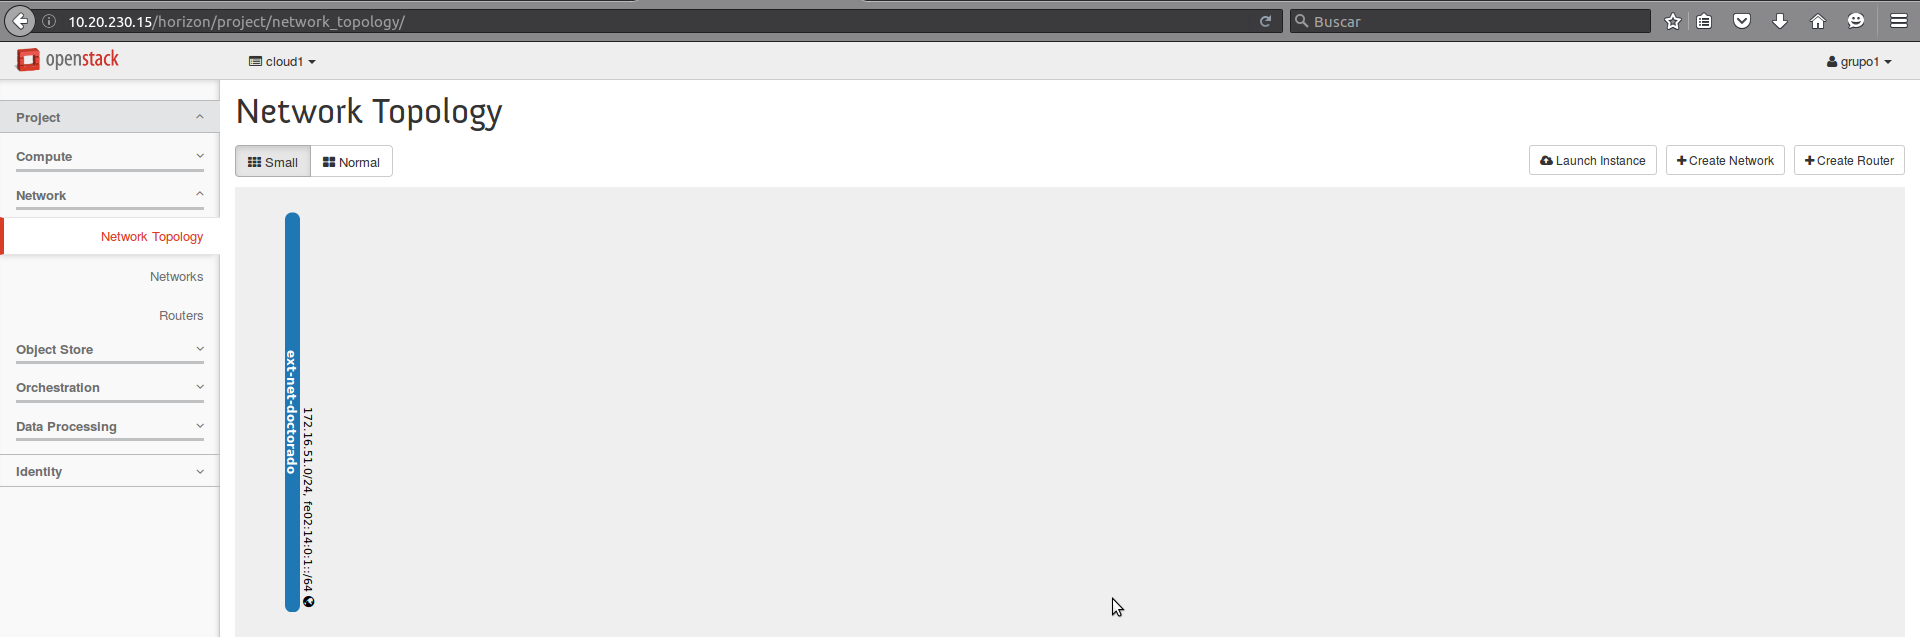
\includegraphics[scale=0.28]{OpenStackInicial}   % Scale se utiliza para cambiar el tamaño de la imagen
	\caption{Estado inicial del OpenStack} \label{fig:Elementos}
\end{figure}


Se procede a lanzar el Stack:\\


\begin{figure}[ht] % Es preferible verificar la documentación para que la imagen quede correctamente segun el parámetro entre []
	\centering
	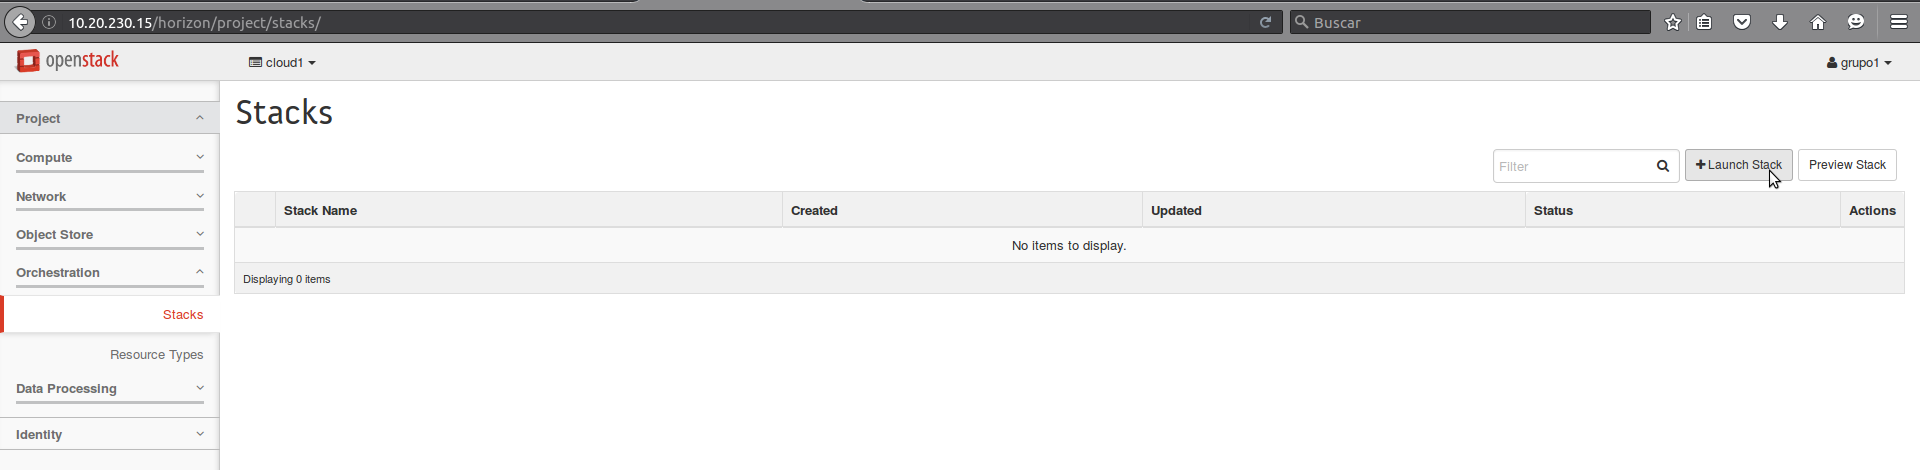
\includegraphics[width=15cm,height=4.5cm]{OpenStackLaunchStacks}   % Scale se utiliza para cambiar el tamaño de la imagen
	\caption{lanzamiento del Stack} \label{fig:Elementos}
\end{figure}

Se lanza el fichero \texttt{\href{https://github.com/wilrilo/talleres/blob/master/file/taller1/router.yaml}{router.yaml}}:\\


\begin{figure}[ht] % Es preferible verificar la documentación para que la imagen quede correctamente segun el parámetro entre []
	\centering
	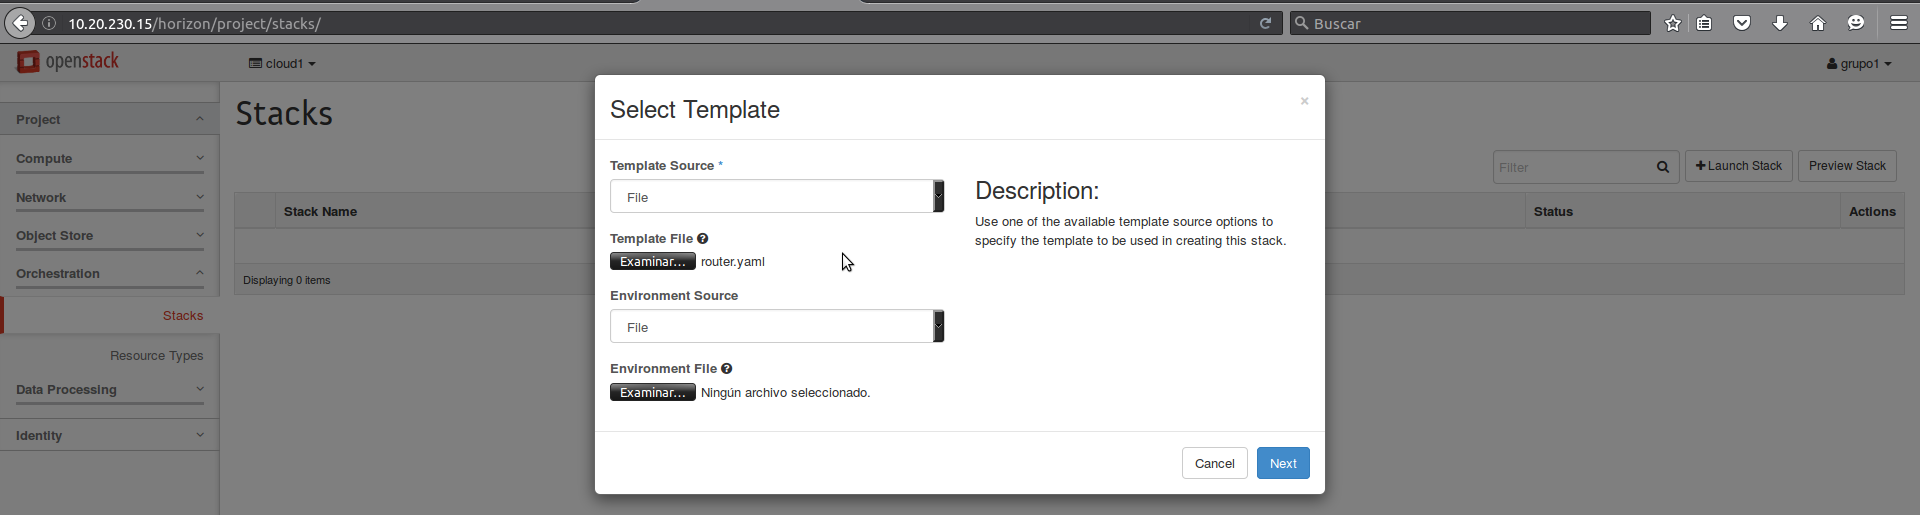
\includegraphics[width=15cm,height=4.5cm]{OpenStackRouteryaml}   % Scale se utiliza para cambiar el tamaño de la imagen
	\caption{Lanzamiento del fichero} \label{fig:Elementos}
\end{figure}

\begin{figure}[ht] % Es preferible verificar la documentación para que la imagen quede correctamente segun el parámetro entre []
	\centering
	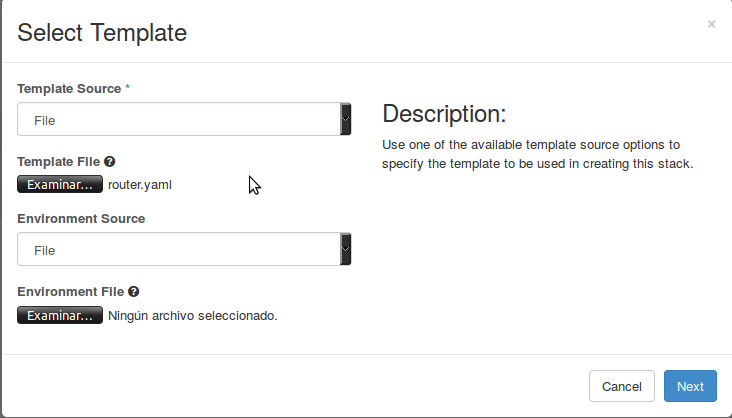
\includegraphics[scale=0.4]{OpenStackRouteryaml2}   % Scale se utiliza para cambiar el tamaño de la imagen
	\caption{ventana para lanzar archivos}
	 \label{fig:Elementos}
\end{figure}

\newpage

Se verifica la creación del Stack: \\



\begin{figure}[ht] % Es preferible verificar la documentación para que la imagen quede correctamente segun el parámetro entre []
	\centering
	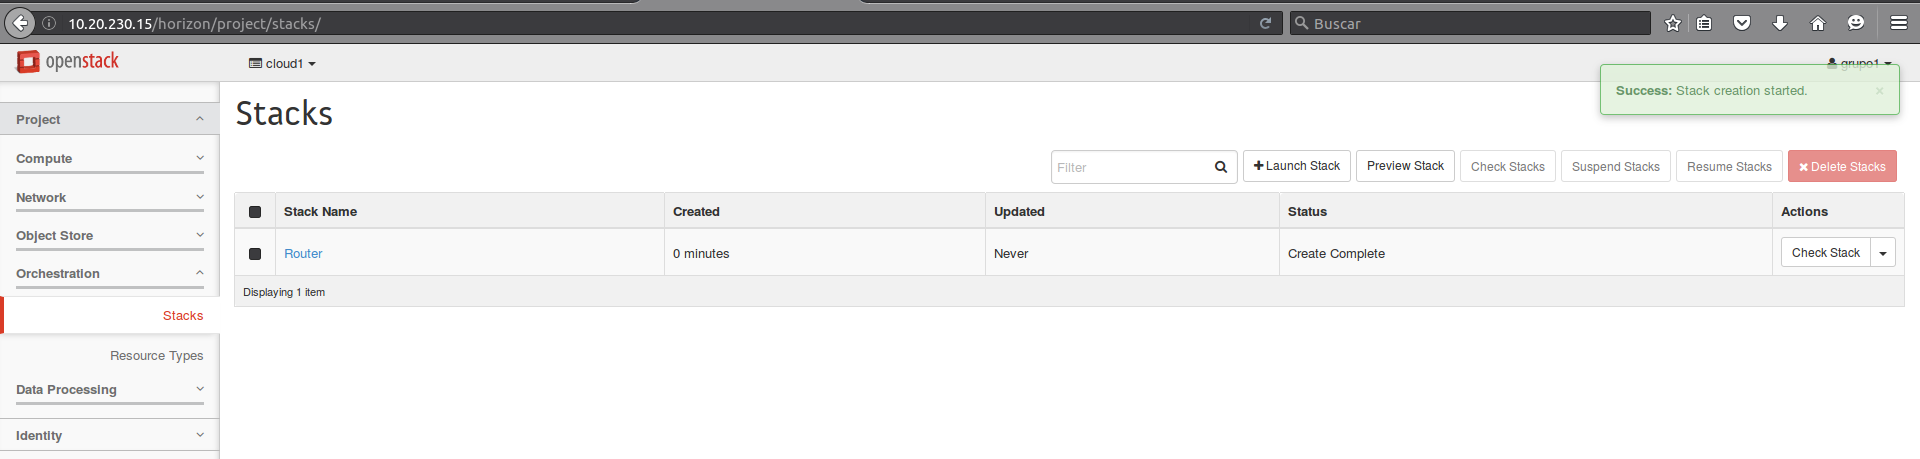
\includegraphics[scale=0.3]{vericrearouter}   % Scale se utiliza para cambiar el tamaño de la imagen
	\caption{Creación del  Stack} \label{fig:Elementos}
\end{figure}

Verificación de Router creado:\\


\begin{figure}[ht] % Es preferible verificar la documentación para que la imagen quede correctamente segun el parámetro entre []
	\centering
	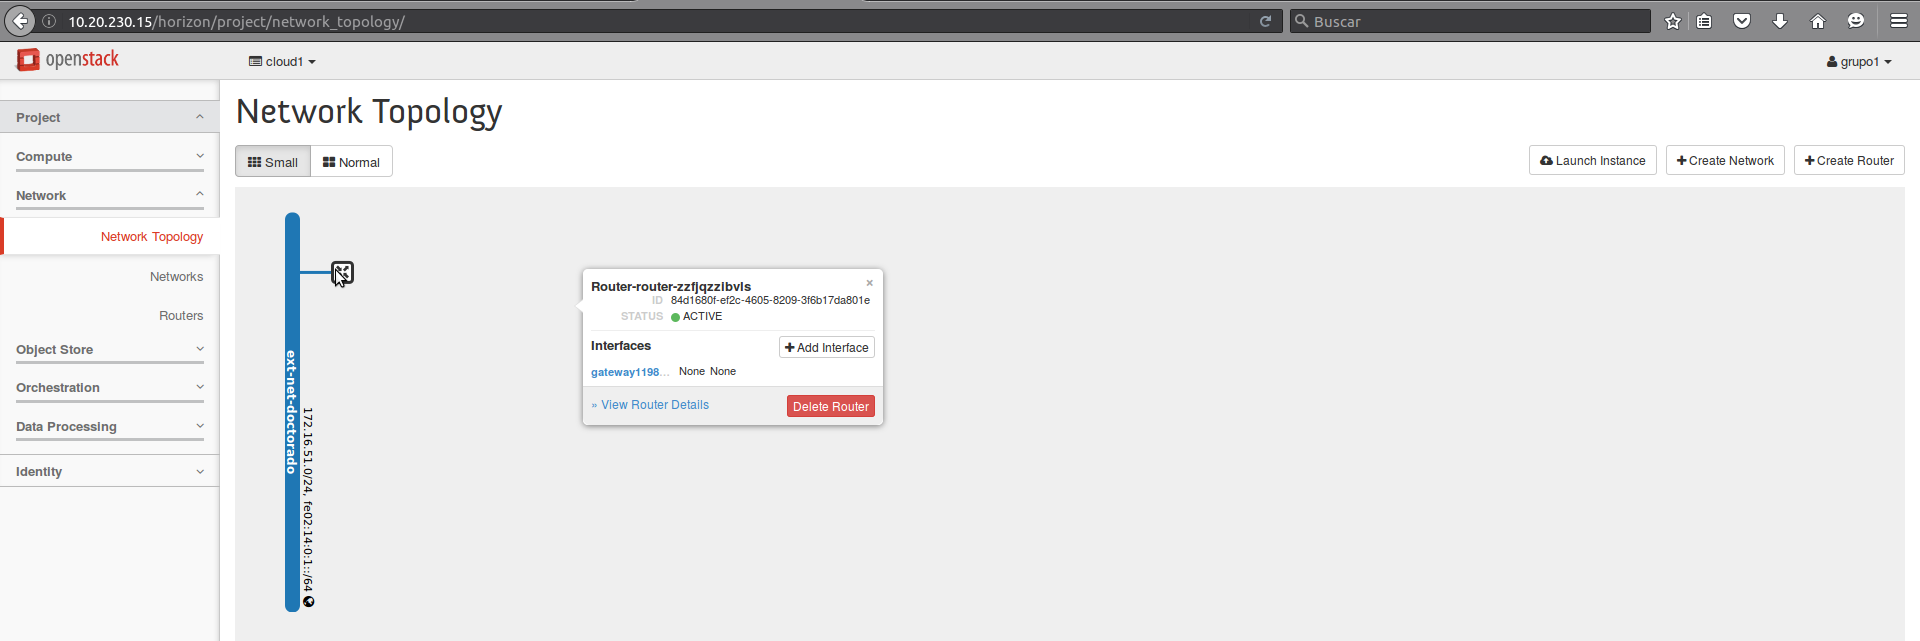
\includegraphics[scale=0.3]{RouterCreated}   % Scale se utiliza para cambiar el tamaño de la imagen
	\caption{Topología donde se observa el router creado} \label{fig:Elementos}
\end{figure}
\newpage
Detalles del Router:

\begin{figure}[ht] % Es preferible verificar la documentación para que la imagen quede correctamente segun el parámetro entre []
	\centering
	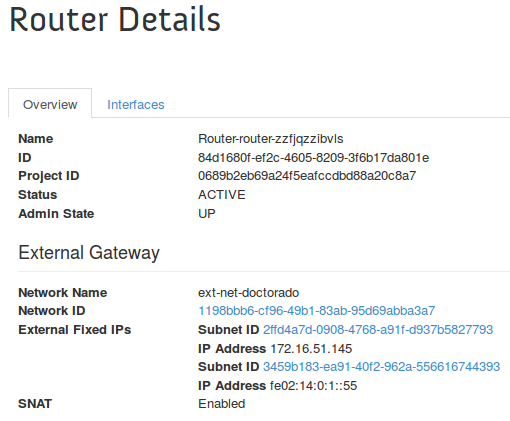
\includegraphics[scale=0.34]{Router}   % Scale se utiliza para cambiar el tamaño de la imagen
	\caption{Descripción de los detalles del router} \label{fig:Elementos}
\end{figure}


\item Crear un archivo denominado “\texttt{\href{https://github.com/wilrilo/talleres/blob/master/file/taller1/network.yaml}{network.yaml}}” con el siguiente contenido y ejecutar la plantilla.


\begin{small}
	\begin{lstlisting}[frame=single,style=base]	
heat_template_version: 2013-05-23

description: This template deploys a router with a port in the public interface

parameters:

private_network_cidr:
type: string
label: Private network CIDR
description: Private Network CIDR
default: 192.168.200.0/24

resources:

private_network:
type: OS::Neutron::Net

private_subnet:
type: OS::Neutron::Subnet
properties:
network_id: { get_resource: private_network }
cidr: {get_param: private_network_cidr}
dns_nameservers:
- 8.8.8.8

	
	\end{lstlisting}
\end{small}

Se comienza lanzando un Stack:\\


\begin{figure}[H] % Es preferible verificar la documentación para que la imagen quede correctamente segun el parámetro entre []
	\centering
	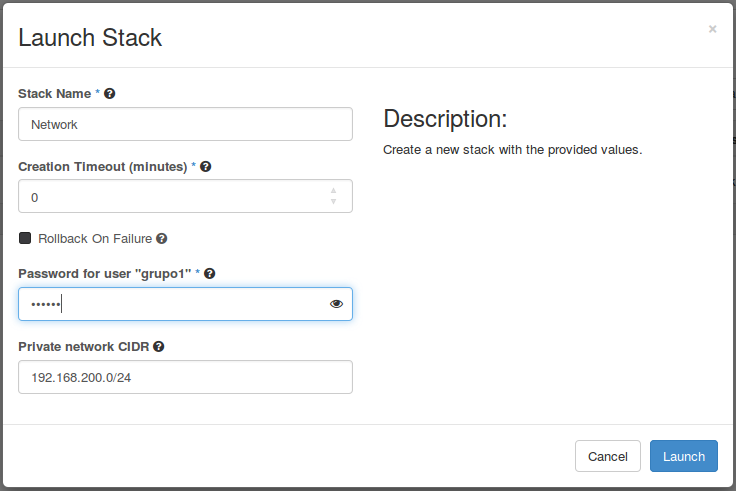
\includegraphics[scale=0.2]{Network}   % Scale se utiliza para cambiar el tamaño de la imagen
	\caption{Ventana para lanzar el  Stack} \label{fig:Elementos}
\end{figure}

Se verifica la creación correcto del Stack:\\



\begin{figure}[ht] % Es preferible verificar la documentación para que la imagen quede correctamente segun el parámetro entre []
	\centering
	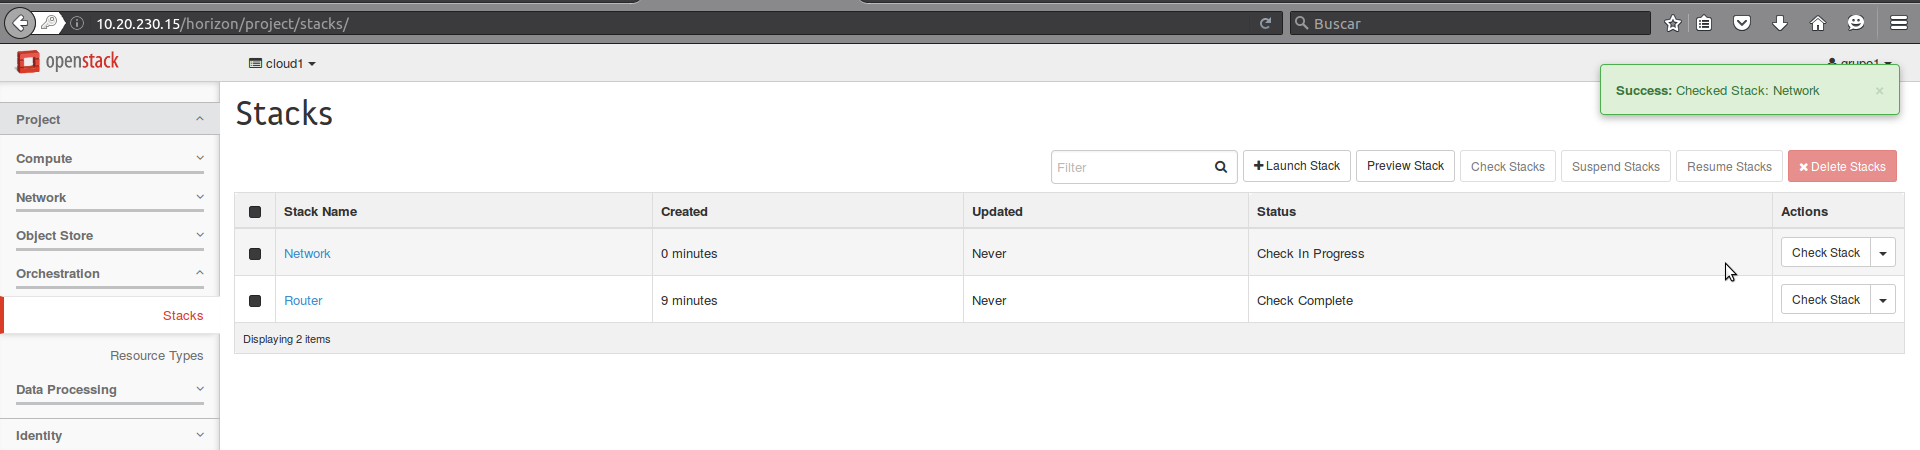
\includegraphics[scale=0.35]{Created}   % Scale se utiliza para cambiar el tamaño de la imagen
	\caption{Verificación de la creación del Stack} \label{fig:Elementos}
\end{figure}

Nos dirigimos a redes (Networks) para  verificar la correcta creación de la red: 

\begin{figure}[ht] % Es preferible verificar la documentación para que la imagen quede correctamente segun el parámetro entre []
	\centering
	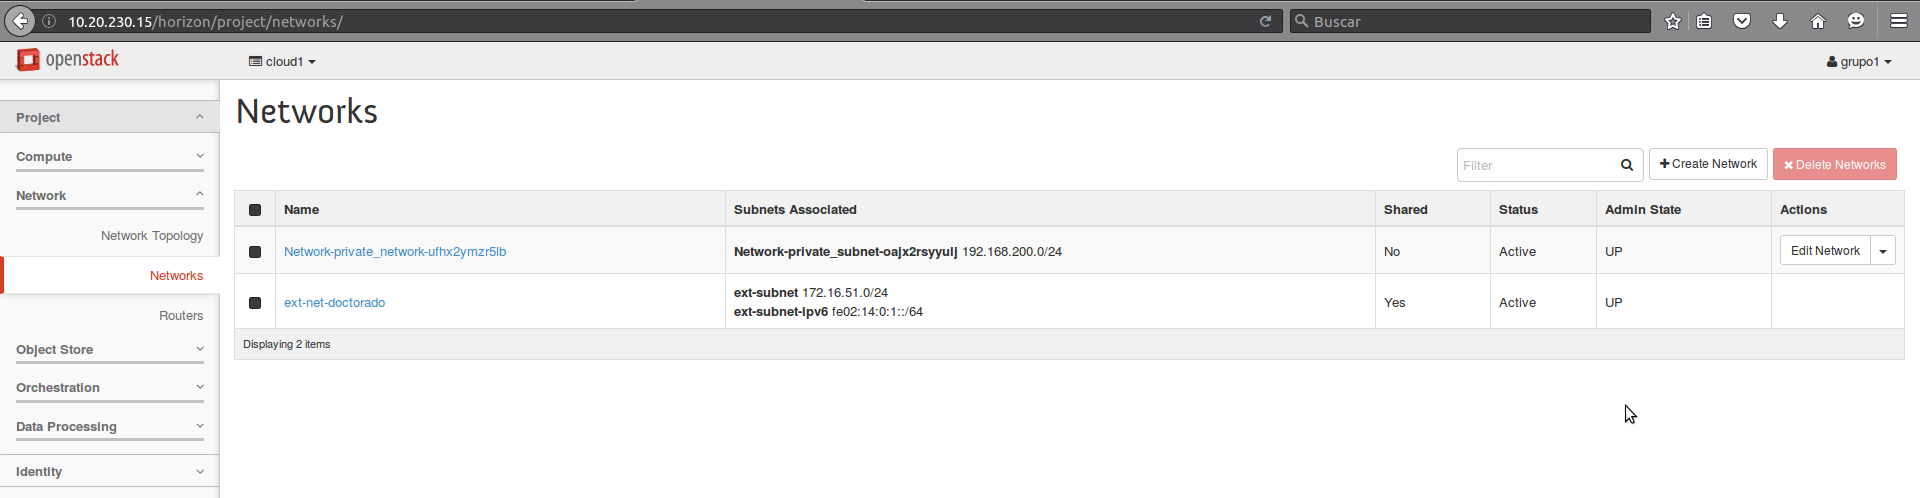
\includegraphics[scale=0.35]{RedesCreadas}   % Scale se utiliza para cambiar el tamaño de la imagen
	\caption{Verificación de la creación de la red} \label{fig:Elementos}
\end{figure}

\item Finalmente en topologia de red vemos el router y la red creadas anteriormente: \\




\begin{figure}[H] % Es preferible verificar la documentación para que la imagen quede correctamente segun el parámetro entre []
	\centering
	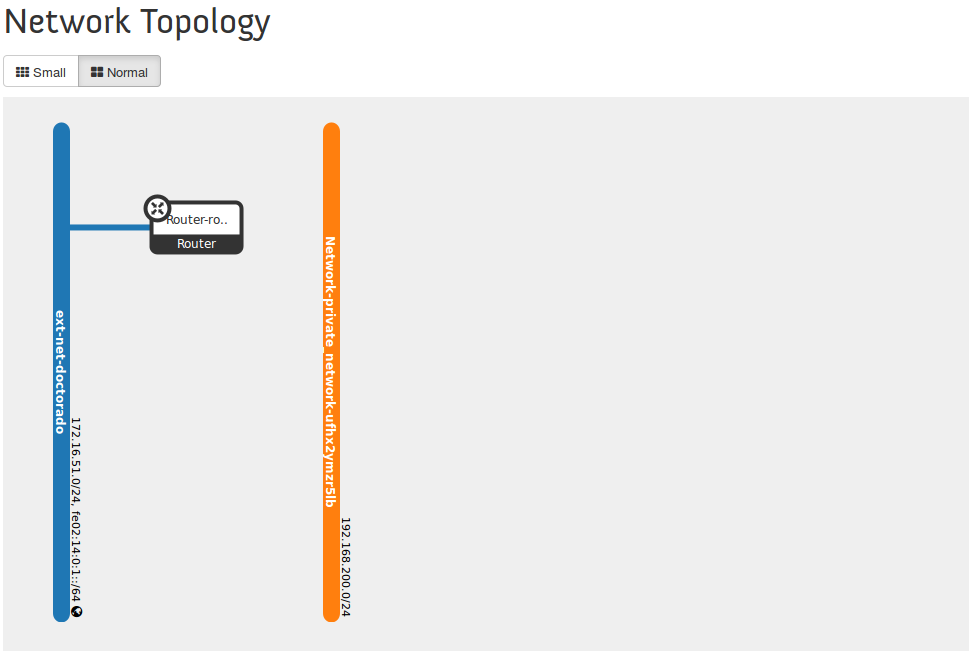
\includegraphics[scale=0.32]{Resultado}   % Scale se utiliza para cambiar el tamaño de la imagen
	\caption{Topología de la red} \label{fig:Elementos}
\end{figure}

\item Eliminar las pilas previamente creadas. 



\item 	Crear un archivo denominar “\texttt{\href{https://github.com/wilrilo/talleres/blob/master/file/taller1/complete-network.yaml}{complete-network.yaml}}” con el siguiente contenido y ejecutar la plantilla. En este paso, se va a crear un router, una red privada, y se le va a asignar un puerto al router dentro de esa red:


\begin{small}
	\begin{lstlisting}[frame=single,style=base]	
	
	
	heat_template_version: 2013-05-23
	
	description: This template deploys a router with a port in the public interface
	
	parameters:
	
	public_network:
	type: string
	label: Public network name or ID
	description: Public network with floating IP addresses.
	default: ext-net-doctorado
	
	private_network_cidr:
	type: string
	label: Private network CIDR
	description: Private Network CIDR
	default: 192.168.200.0/24
	
	resources:
	
	router:
	type: OS::Neutron::Router
	properties:
	external_gateway_info:
	network: { get_param: public_network }
	
	private_network:
	type: OS::Neutron::Net
	
	private_subnet:
	type: OS::Neutron::Subnet
	properties:
	network_id: { get_resource: private_network }
	cidr: {get_param: private_network_cidr}
	dns_nameservers:
	- 8.8.8.8
	
	router-interface:
	type: OS::Neutron::RouterInterface
	properties:
	router_id: { get_resource: router }
	subnet: { get_resource: private_subnet }
	
	
	\end{lstlisting}
\end{small}

 lanzamos el Stack:
 
 \begin{figure}[H] % Es preferible verificar la documentación para que la imagen quede correctamente segun el parámetro entre []
	\centering
	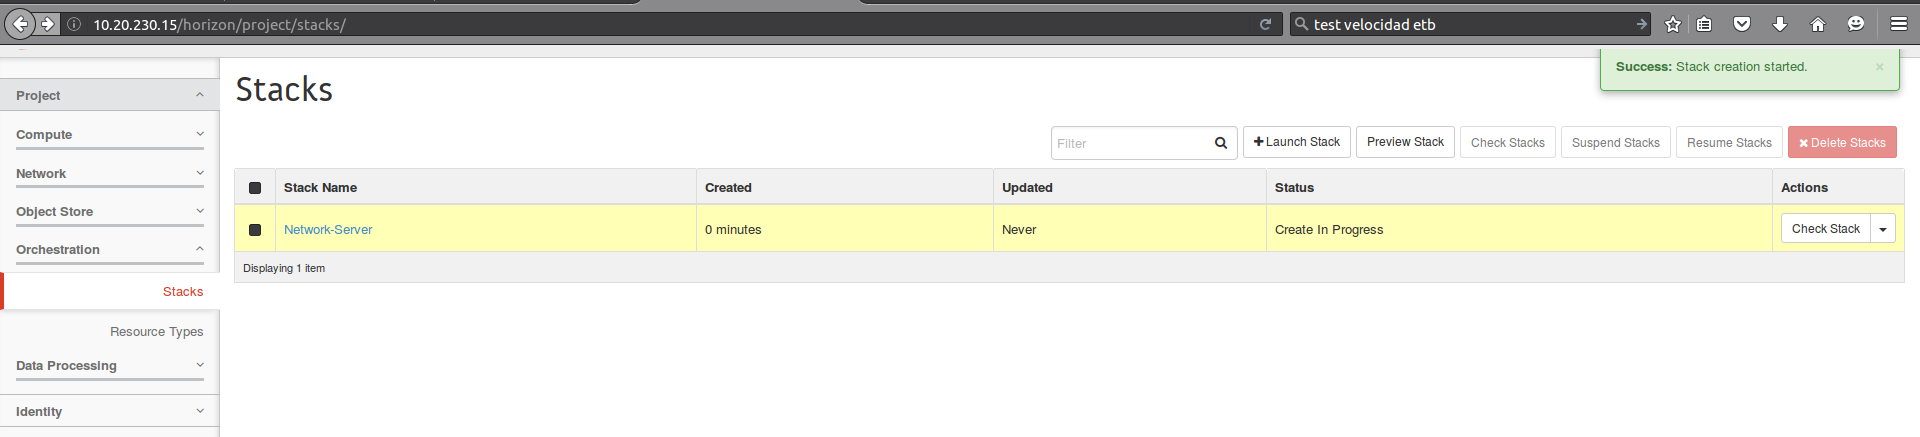
\includegraphics[scale=0.2]{Stack}   % Scale se utiliza para cambiar el tamaño de la imagen
	\caption{Lanzamiento del Stack} \label{fig:Elementos}
\end{figure}
Se verifica la topología de la red:


 \begin{figure}[ht] % Es preferible verificar la documentación para que la imagen quede correctamente segun el parámetro entre []
 	\centering
 	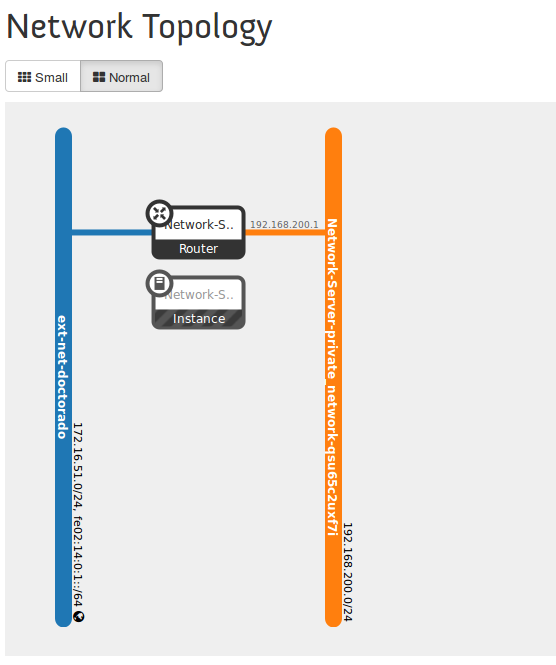
\includegraphics[scale=0.4]{NetworkTopologyRunning}   % Scale se utiliza para cambiar el tamaño de la imagen
 	\caption{Topología de la red} \label{fig:Elementos}
 \end{figure}
 

 Una vez la infraestructura de red, el siguiente paso es crear servidores. Inicialmente, se desplegará únicamente el servidor con su respectivo grupo de seguridad.  Posteriormente se le configurará en la plantilla el software a instalar y se le asignará un IP flotante.\\
 
 
  \item 	Eliminar las pilas previamente creadas.
  
  \item Crear un archivo denominar “\texttt{\href{https://github.com/wilrilo/talleres/blob/master/file/taller1/network-server.yaml}{network-server.yaml}}” con el siguiente contenido y ejecutar la plantilla. En este paso, se va a crear un router, una red privada, se le va a asignar un puerto al router dentro de esa red, y se va a lanzar una instancia con un grupo de seguridad denominado “\texttt{web\_server\_security\_group}” y una llave “\texttt{cloudapps}” .




\begin{small}
	\begin{lstlisting}[frame=single,style=base]	
heat_template_version: 2013-05-23

description: This template deploys a router, a private network and a single basic server with a security group.

parameters:

public_network:
type: string
label: Public network name or ID
description: Public network with floating IP addresses.
default: ext-net-doctorado

private_network_cidr:
type: string
label: Private network CIDR
description: Private Network CIDR
default: 192.168.200.0/24

image:
type: string
label: Image name or ID
description: Image to be used for compute instance
default: Ubuntu-Server-14.04-CECAD-r20141201

flavor:
type: string
label: Flavor
description: Type of instance (flavor) to be used
default: m1.small


resources:

router:
type: OS::Neutron::Router
properties:
external_gateway_info:
network: { get_param: public_network }

private_network:
type: OS::Neutron::Net

private_subnet:
type: OS::Neutron::Subnet
properties:
network_id: { get_resource: private_network }
cidr: {get_param: private_network_cidr}
dns_nameservers:
- 8.8.8.8

router-interface:
type: OS::Neutron::RouterInterface
properties:
router_id: { get_resource: router }
subnet: { get_resource: private_subnet }

web_server_security_group:
type: OS::Neutron::SecurityGroup
properties:
name: web_server_security_group
rules:
- protocol: tcp
port_range_min: 80
port_range_max: 80
- protocol: tcp
port_range_min: 443
port_range_max: 443
- protocol: icmp
- protocol: tcp
port_range_min: 22
port_range_max: 22

my_keypair:
type: OS::Nova::KeyPair
properties:
name: cloudapps
save_private_key: True

my_instance:
type: OS::Nova::Server
properties:
image: { get_param: image }
flavor: { get_param: flavor }
key_name: { get_resource: my_keypair }
networks:
- network: { get_resource: private_network }
security_groups:
- { get_resource: web_server_security_group }
user_data: |
#!/bin/sh
sudo apt-get -y update && sudo apt-get -y install apache2 && sudo service apache2 restart
user_data_format: RAW

outputs:
my_instance_name:
description: Name of the instance
value: { get_attr: [my_instance, name] }
my_instance_ip:
description: IP address of the instance
value: { get_attr: [my_instance, first_address] }

	
	\end{lstlisting}
\end{small}



Lanzamiento del Stack:
 \begin{figure}[H] % Es preferible verificar la documentación para que la imagen quede correctamente segun el parámetro entre []
 	\centering
 	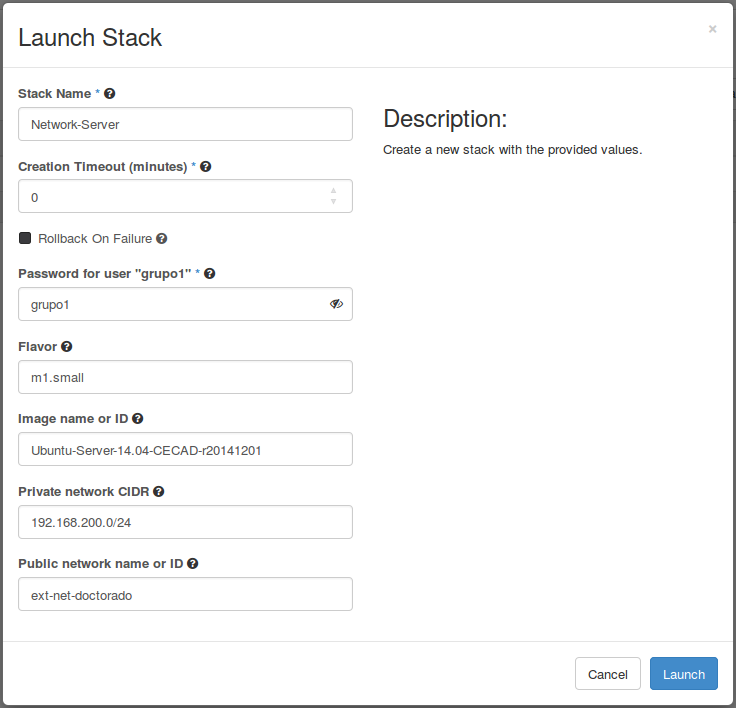
\includegraphics[scale=0.3]{LaunchStack}   % Scale se utiliza para cambiar el tamaño de la imagen
 	\caption{Lanzamiento del Stack} \label{fig:Elementos}
 \end{figure}


 \begin{figure}[H] % Es preferible verificar la documentación para que la imagen quede correctamente segun el parámetro entre []
 	\centering
 	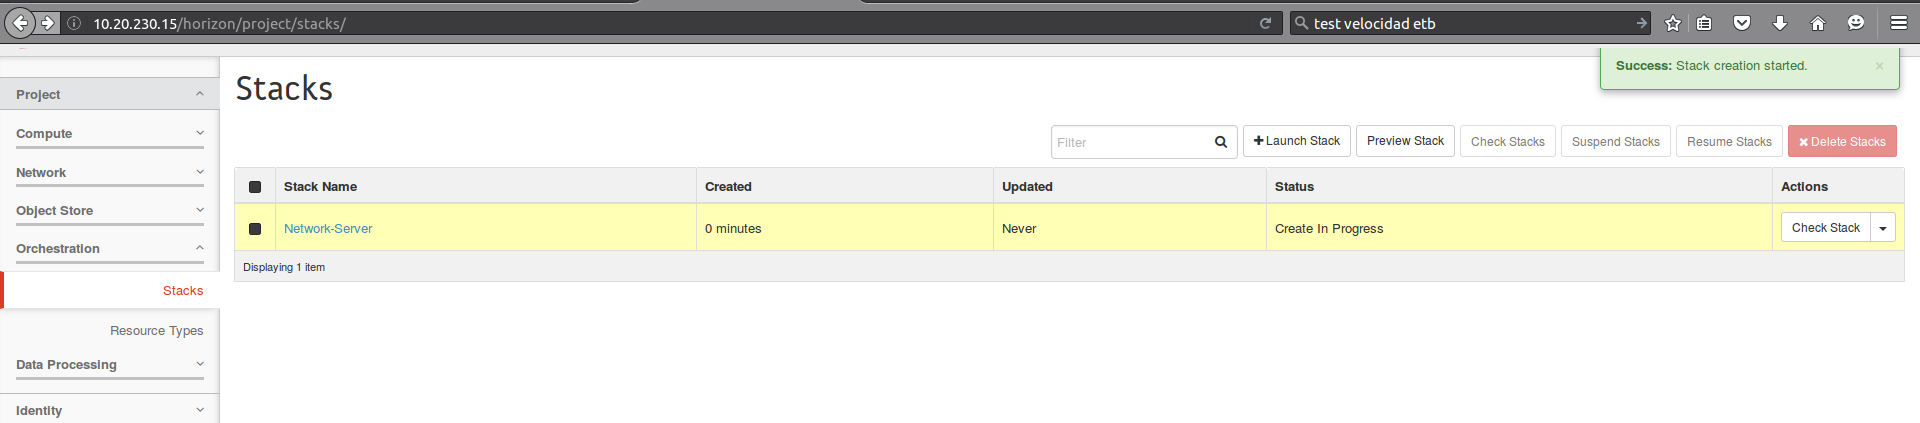
\includegraphics[scale=0.34]{StackN}   % Scale se utiliza para cambiar el tamaño de la imagen
 	\caption{Lanzamiento del Stack} \label{fig:Elementos}
 \end{figure}
 
 Se verifica la creación del Stack en la topologia de la red
 
  \begin{figure}[ht] % Es preferible verificar la documentación para que la imagen quede correctamente segun el parámetro entre []
  	\centering
  	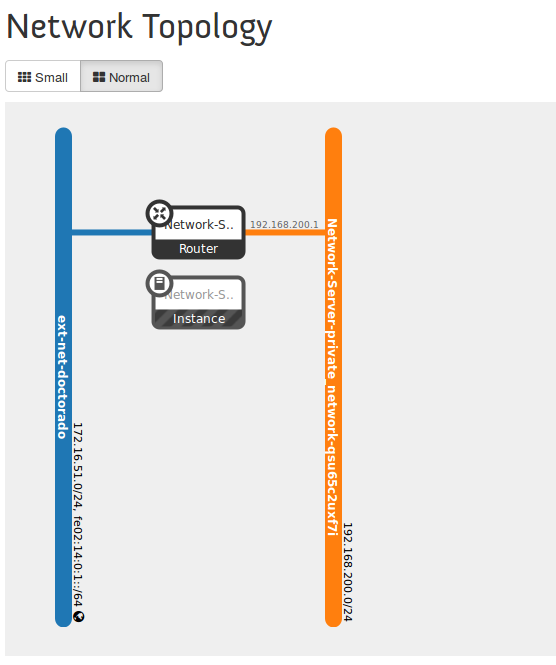
\includegraphics[scale=0.3]{NetworkTopologyRunning}   % Scale se utiliza para cambiar el tamaño de la imagen
  	\caption{Verificación de la creación del Stack} \label{fig:Elementos}
  \end{figure}
 
 Topología de la red:\\
 
 
   \begin{figure}[ht] % Es preferible verificar la documentación para que la imagen quede correctamente segun el parámetro entre []
   	\centering
   	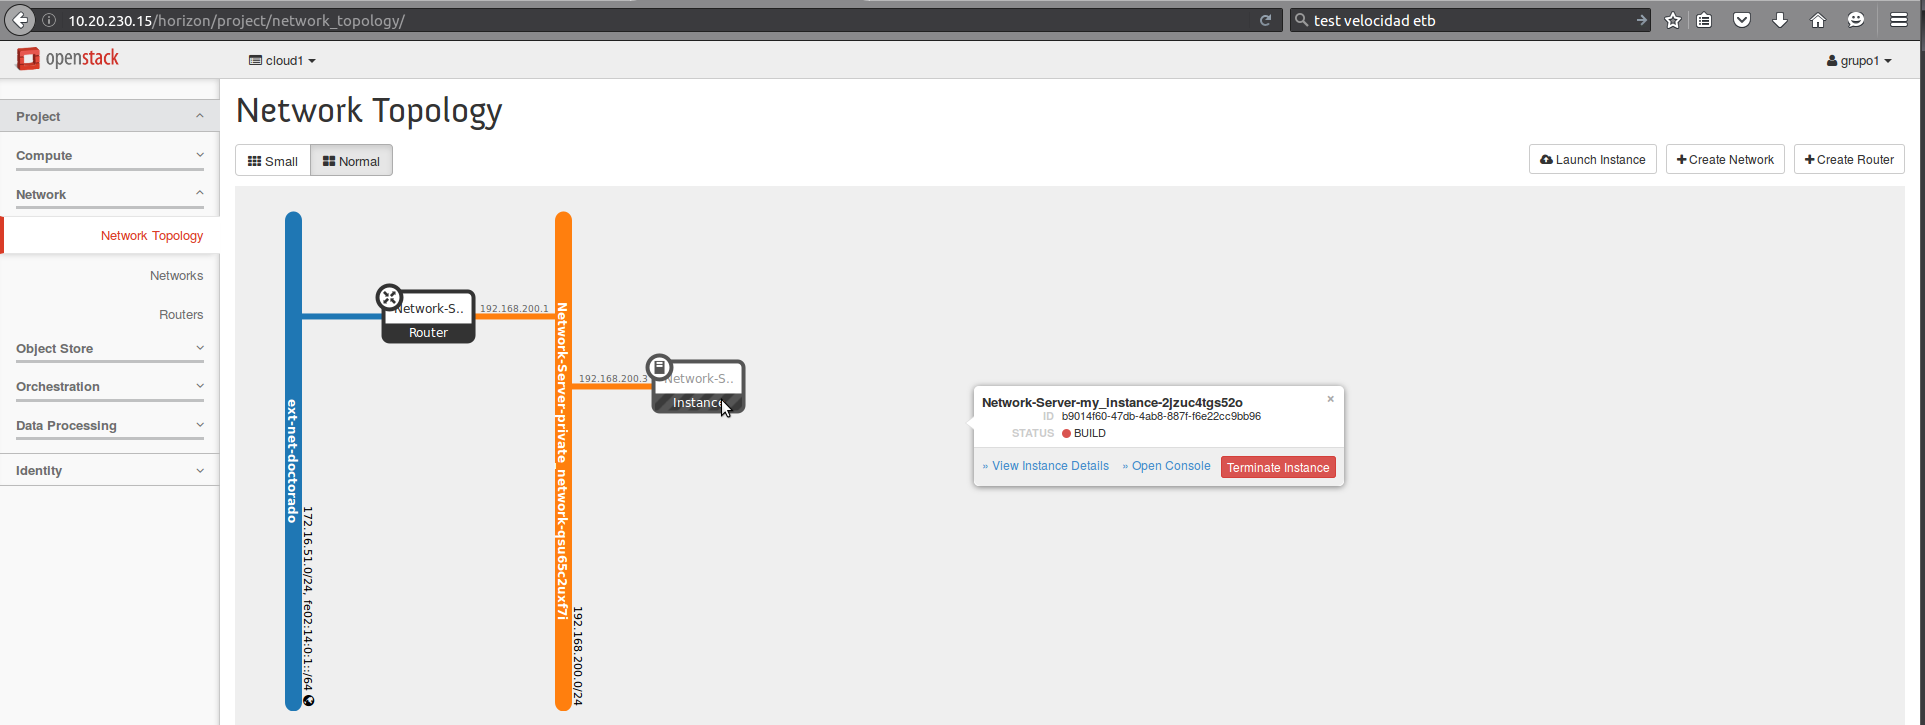
\includegraphics[scale=0.18]{BuildingInstance}   % Scale se utiliza para cambiar el tamaño de la imagen
   	\caption{Topología de la red} \label{fig:Elementos}
   \end{figure}
   
 Después de creada la instancia se abre la consola:
   \begin{figure}[H] % Es preferible verificar la documentación para que la imagen quede correctamente segun el parámetro entre []
   	\centering
   	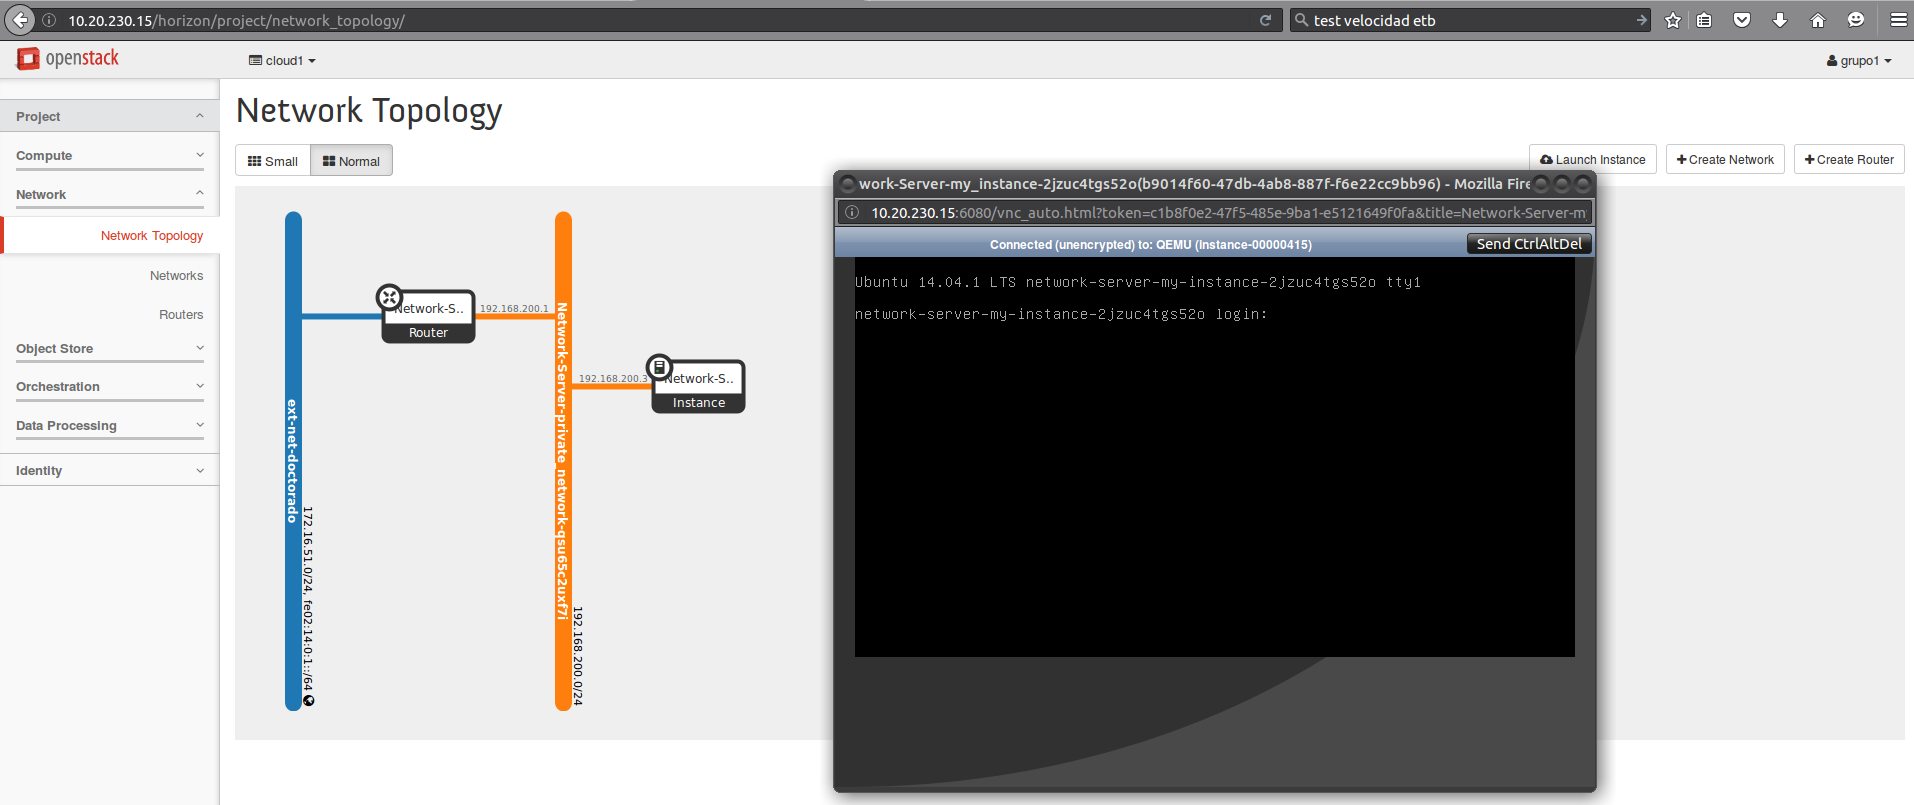
\includegraphics[scale=0.3]{ConsoleNetworkInstance}   % Scale se utiliza para cambiar el tamaño de la imagen
   	\caption{Apertura de la consola en la instancia} \label{fig:Elementos}
   \end{figure}
\item Se le  Asigna una IP Flotante a la instancia: 172.18.51.148:

\begin{figure}[ht] % Es preferible verificar la documentación para que la imagen quede correctamente segun el parámetro entre []
	\centering
	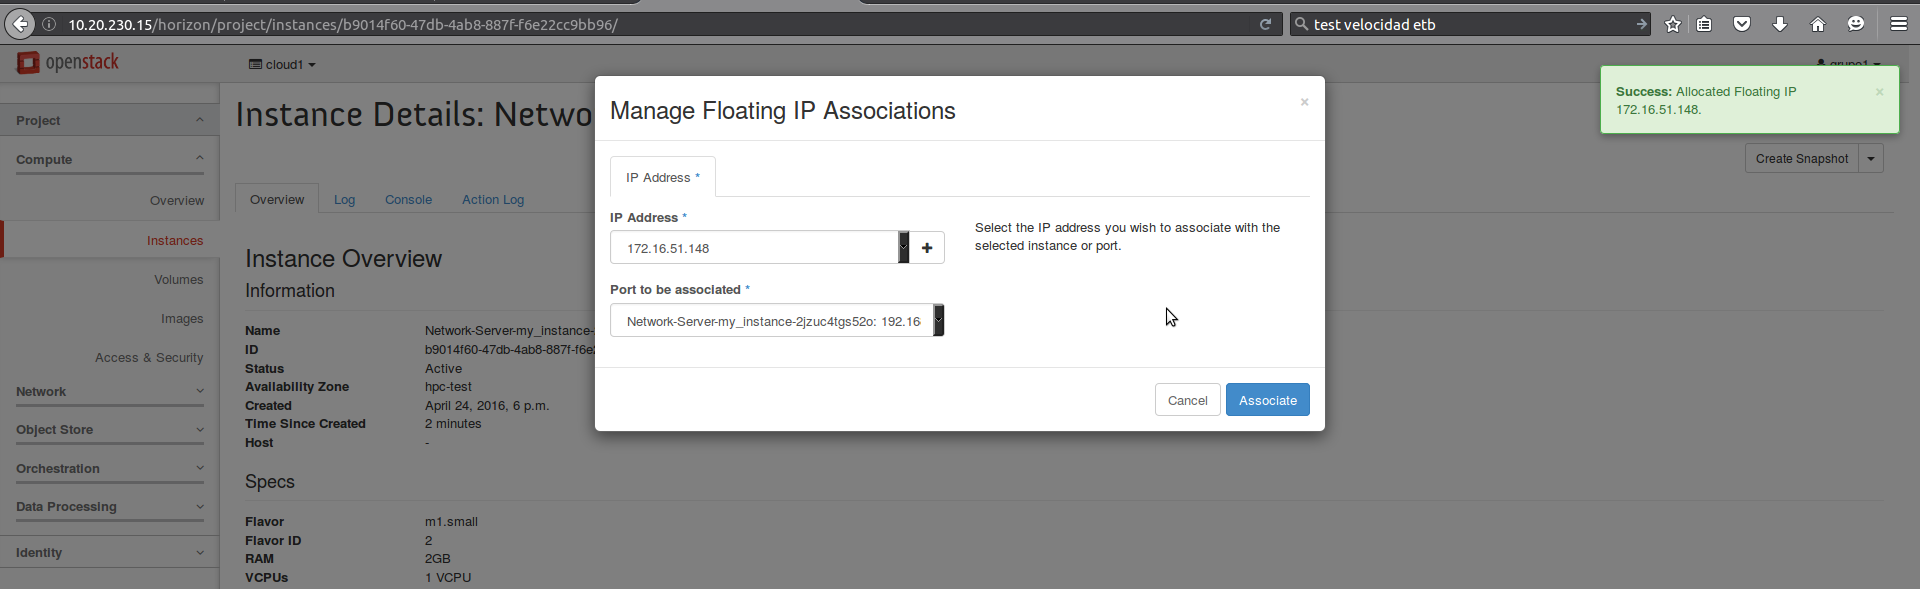
\includegraphics[scale=0.35]{IPFlotantealainstancia}   % Scale se utiliza para cambiar el tamaño de la imagen
	\caption{Asignación de una IP flotante} \label{fig:Elementos}
\end{figure}


A continuación se muestran los resultados de la Instancia 


\begin{figure}[H] % Es preferible verificar la documentación para que la imagen quede correctamente segun el parámetro entre []
	\centering
	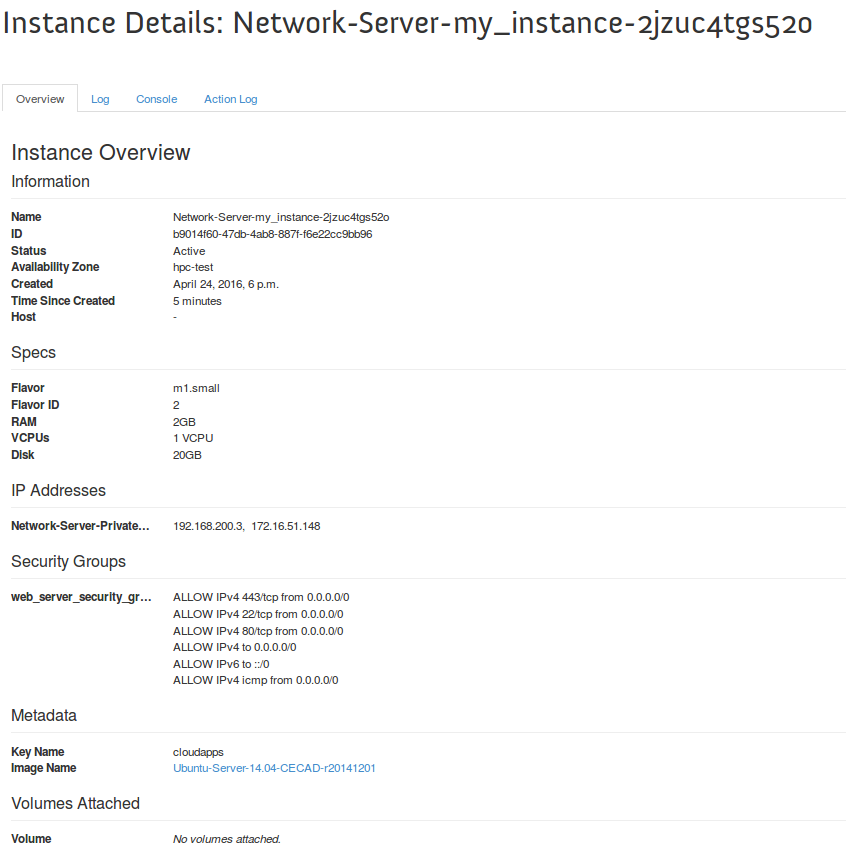
\includegraphics[scale=0.4]{InstanciaconIPflotante}   % Scale se utiliza para cambiar el tamaño de la imagen
	\caption{Resultados de la Instancia} \label{fig:Elementos}
\end{figure}
\newpage
\item Se realiza un Ping hacia la IP Flotante de la Instancia creada:

\begin{figure}[H] % Es preferible verificar la documentación para que la imagen quede correctamente segun el parámetro entre []
	\centering
	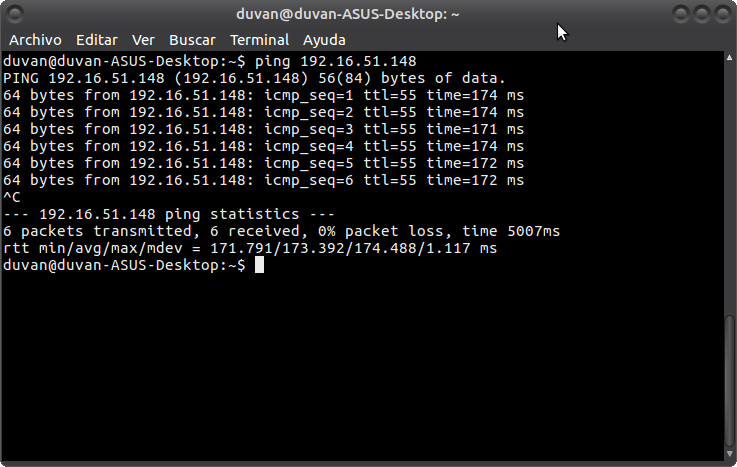
\includegraphics[scale=0.33]{PingalaIPFlotante}   % Scale se utiliza para cambiar el tamaño de la imagen
	\caption{Verificación del funcionamiento mediante un ping} \label{fig:Elementos}
\end{figure}

\section{Bibliografía}

\begin{itemize}
	\item \href{http://vmartinezdelacruz.com/en-pocas-palabras-como-funciona-openstack/}{http://vmartinezdelacruz.com/en-pocas-palabras-como-funciona-openstack/}
	\item \href{https://www.openstack.org/
		}{https://www.openstack.org/
		}
	\item \href{http://www.ubuntu.com/cloud/openstack
		}{http://www.ubuntu.com/cloud/openstack
		}
	
\end{itemize}
	

\end{enumerate}

	
\end{document}
